\chapter{Autonomous Target Following System}
This chapter presents a vision-based target tracking and following system using a monocular camera on an Unmanned Aerial System (UAS). The Recursive-RANSAC (R-RANSAC) tracker tracks multiple moving objects in the camera field of view and the proposed controller is capable of following a particular target selected by a user while keeping the target in the center of the image. The main contribution of this work is that multiple objects can be tracked without imposing restrictions such as color, shape, etc. Also, the hardware test shows that the system is able to follow a target autonomously in a real-world outdoor environment.

\section{System Overview}
\begin{figure}[htbp]
	\centering
	\framebox{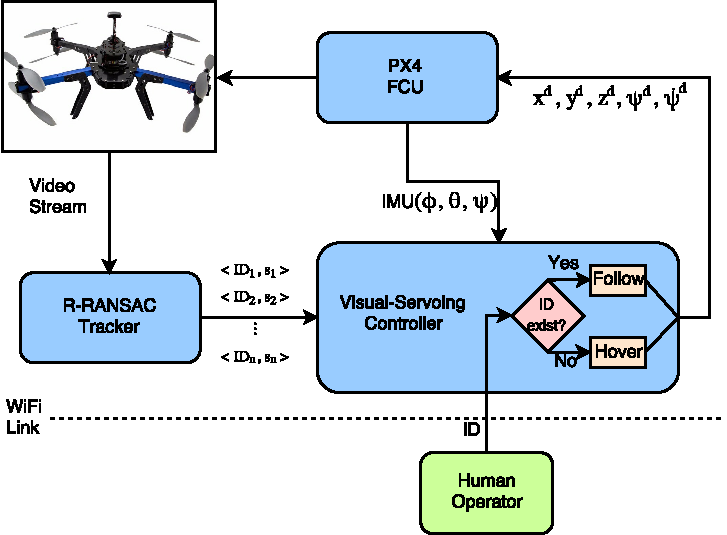
\includegraphics[width=0.6\textwidth]{images/chapter3/system_diagram.pdf}}
	\caption{System Architecture. The R-RANSAC tracker produces a set of target ID numbers and corresponding pixel locations. The visual-servoing controller outputs the desired position, heading, and yaw rate based on the pixel location of the requested target.}
	\label{system}
\end{figure}
The R-RANSAC tracker and the visual-servoing controller are major subsystems as shown in Figure \ref{system} and they communicate using the Robot Operating System (ROS) framework. The Pixhawk flight controller is used with the PX4 firmware for the autopilot. The R-RANSAC tracker is responsible for tracking moving objects in the image sequence and outputs a vector of normalized image coordinates with unique ID assigned to each track. Let the normalized pixel coordinates be defined as 
\begin{equation}
s = [\epsilon_x, \epsilon_y]
\end{equation} where $\epsilon_x$, $\epsilon_y$ are normalized pixel coordinates. Combined with IDs, a vector of track information is defined as 
\begin{equation}
T = [<ID_1, s_1>, <ID_2, s_2>, \dots, <ID_n, s_n>].
\end{equation}
The human operator assigns which target the UAV is to follow by sending a target ID number using the ground station. The controller checks to see if the target with the same ID given by the human operator exists among tracks. If the target exists, the controller keeps the target in the center of the image by commanding yaw rate and forward, backward motion of the UAV. Otherwise, the controller holds the UAV's current position until it receives another target ID existing among tracks. 

\section{Recursive-RANSAC Tracker}
This section describes the visual detection and tracking framework. The objective of the visual tracker is to reliably track all targets in the field of view such that the ground operator can select a desired ID number for visual servoing. All elements of target tracking are required to be autonomous, without a priori knowledge of the number of targets in the field of view. A key requirement is track continuity (persistent track ID numbers) in order for the system to achieve good following performance. An ID-loss event requires the ground operator to select the new target ID when the track is re-initialized which leads to undesirable flight behavior. No detection aids such as color segmentation or truth data are available to the controller, meaning that target detection and state estimation must be robust in standard flight environments.
\begin{figure}[htbp]
	\centering
	\framebox{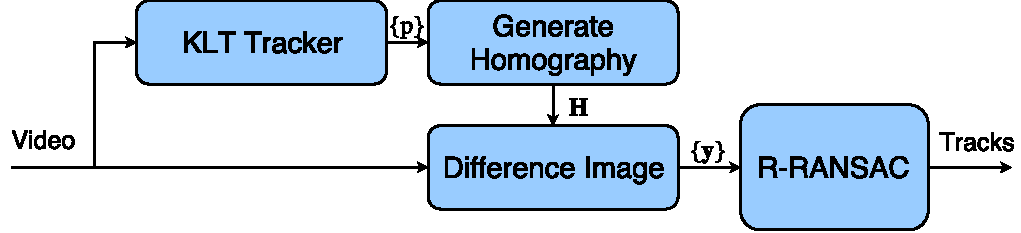
\includegraphics[width=0.8\textwidth]{images/chapter3/tracker_diagram.pdf}}
	\caption{This figure illustrates the detection framework used to generate measurements used by R-RANSAC. The KLT tracker creates point correspondences between frames which are used to calculate a homography. The difference image detects motion in the frame and creates position measurements.}
	\label{visual_tracking}
\end{figure}

Difference imaging reveals motion in the field of view by warping the previous image into the current timestep and comparing the two frames. This approach was used because it tends to be more robust in the presence of noisy homography transforms and image imperfections experienced by rolling shutter cameras in the presence of vibration. Our flight demonstration used entry-level hardware such as a webcam without gimbal stabalization.

This form of motion detection requires knowledge of the homography as seen in Figure \ref{visual_tracking}. The KLT algorithm is used to create point correspondences accross the image and the homography is generated from these points using a RANSAC method.

R-RANSAC is an MTT algorithm that generates many hypothesis trajectories based upon an assumed dynamic model of the targets and the set of recent measurements. By elevating models that surpass a threshold of inlier measurements, the algorithm is capable of tracking many targets with missed detections in clutter \cite{Niedfeldt2014}.

For each new scan of measurements, the ones that are inliers to existing models are used to perform a Kalman update using a probabalistic data association (PDA) filter. For each measurement that is an outlier to all existing models, a new model is generated by sampling trajectories based on the recent history of recieved measurements. The sampled trajectory with the most support (having the most inliers) is selected to define the new model and the inlier measurements are used to estimate the target state estiamate and error covariance for the current timestep. Additional operations perform model merging and pruning in order to eliminate unlikely models.

By using the difference image measurements and R-RANSAC, track ID numbers are produced for targets in the field of view and can be used for visual servoing operations.

\section{UAV Control}
The visual tracking system in the previous section provides the control algorithm with a vector of normalized image coordinates for every track in the camera field of view. The control algorithm activates follow mode when there exists a target with the ID that a human operator has assigned for following. When the given ID is not found in the vector that the tracker provides, the control algorithm commands the UAV to hold its position until another target ID that exists among the tracks is assigned to follow. In this section, the control algorithm is described in more detail.

\subsection{Coordinate Frame Convention}
Before giving a detailed explanation of the control algorithm, it is worth clarifying our assumptions and the coordinate frames used. 

First, an East-North-Up (ENU) coordinate frame is used as opposed to the common North-East-Down (NED) coordinates for UAV in order to match the frame convention used in the \texttt{mavros} package in ROS \cite{mavros}. Let $\mathcal{F}^i$ be the inertial frame, which in this case coincides with the ENU frame, and let $\mathcal{F}^v$ be the vehicle frame that is translated to the UAV center of mass, with the same orientation as $\mathcal{F}^i$. Vehicle-1 frame, $\mathcal{F}^{v1}$ indicates the frame that is only rotated about the $z$-axis of $\mathcal{F}^{v}$ by $\psi$, the heading angle of the multirotor. The rotation matrix from $\mathcal{F}^v$ to $\mathcal{F}^{v1}$ can be expressed as $R^{v1}_v$. Other involved frames are optical, camera, and body frames expressed as $\mathcal{F}^o$, $\mathcal{F}^c$, $\mathcal{F}^b$, respectively. 

Second, a flat-earth model is used to properly scale the target position relative to the camera in $\mathcal{F}^{v1}$ and we have access to the correct altitude information. 

Third, the displacement between the center of mass of the UAV and the focal point of camera is ignored since it is negligible compared to the distance between the camera and the target. 

Fourth, we rely on GPS position controller on autopilot. The visual-servoing controller in this paper computes the desired multirotor position in order to follow the target and send the position command to the autopilot.

\subsection{Forward and heading motion control}
\begin{figure}[thpb]
	\centering
	\framebox{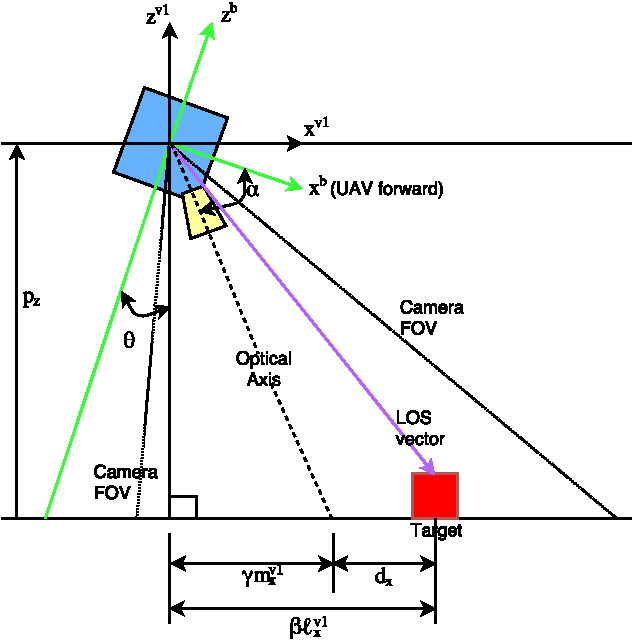
\includegraphics[width=0.5\textwidth]{images/side_view_45deg_2.pdf}}
	\caption{Side view of the multirotor.}
	\label{side_view}
\end{figure}
The first step of the motion control is to transform the line of sight (LOS) vector to the target in $\mathcal{F}^o$ into $\mathcal{F}^{v1}$. Let 
\begin{equation}
\mathbf{\ell}^o=[\epsilon_x^o, \epsilon_y^o, 1]^\top
\end{equation} where $\ell^o$ is the normalized line of sight vector in $\mathcal{F}^o$ and its third element 1 indicates the focal length of the camera in the normalized image. Let also the unit vector along the optical axis in $\mathcal{F}^o$ be defined as 
\begin{equation}
\mathbf{m}^o=[0, 0, 1]^\top.
\end{equation}
By applying sequential transformations to $\ell^o$ and $\mathbf{m}^o$, we get
\begin{equation}
\mathbf{\ell}^{v1}=R^{v1}_b(\phi,\theta)R^b_c(\alpha)R^c_o\ell^o=[\ell^{v1}_x, \ell^{v1}_y, \ell^{v1}_z]^\top
\end{equation}
\begin{equation}
\mathbf{m}^{v1}=R^{v1}_b(\phi,\theta)R^b_c(\alpha)R^c_o\mathbf{m}^o=[m^{v1}_x, m^{v1}_y, m^{v1}_z]^\top
\end{equation} where $R^b_c$ is a matrix with fixed values depending on how the camera is mounted with respect to $\mathcal{F}^b$, $R^{v1}_b$ is a matrix requiring the roll and pitch angles of the multirotor. The $\ell^{v1}$ is the displacement of the target relative to the multirotor and $\mathbf{m}^{v1}$ is the optical axis in $\mathcal{F}^{v1}$. The LOS vector $\ell^{v1}$ and $\mathbf{m}^{v1}$ do not have proper scalings due to the unknown depth information to the target in $\mathcal{F}^o$, but can be recovered using the altitude of the camera. Let
\begin{equation}
\beta=\frac{p_z}{\ell^{v1}_z}
\end{equation} 
\begin{equation}
\gamma=\frac{p_z}{m^{v1}_z}
\end{equation} where $p_z$ is the altitude of the multirotor. Then, the desired forward position from the current multirotor position can be computed as 
\begin{equation}
d_x=\beta\ell^{v1}_x-\gamma{m}^{v1}_x.
\end{equation}
This $d_x$ may be further broken down into east and north components
\begin{equation}
d_n=d_x\sin(\psi)
\end{equation}
\begin{equation}
d_e=d_x\cos(\psi)
\end{equation} where $\psi$ is the heading of the multirotor. These north and east components are added to the current multirotor east and north positions, and the sum is sent to the autopilot position controller.

It is more suitable to compensate for a target moving horizontally in the image plane by adjusting the multirotor's heading than through lateral motion. Thus, a yaw rate command $\omega_z$ can be computed as 
\begin{equation}
\omega_z=\eta \ell^{v1}_y,
\end{equation} where $\eta>0$ is a control gain.

\section{Experiments and Results}
The main hardware is comprised of a 3DR X8 multirotor platform, a small form factor Gigabyte BRIX GB-BXi7-4500 (no GPU), low-cost USB camera, ELP-USBFHD01M-L21 (rolling shutter), and Pixhawk with PX4 firmware. The proposed system was tested in an outdoor environment to track realistic targets (people). We demonstrate the ability to follow one of the multiple tracked objects while switching the target of interest in real-time. The tracker does not have any prior information about what tracks look like and how they might move. The hardware result shows that the R-RANSAC tracker is able to track multiple targets and to provide the controller with proper coordinates of the targets. It also shows that the controller is able to follow one of the target while keeping it in the camera field of view.
\begin{figure}[htbp]
	\begin{subfigure}{0.48\linewidth}
		\centering
		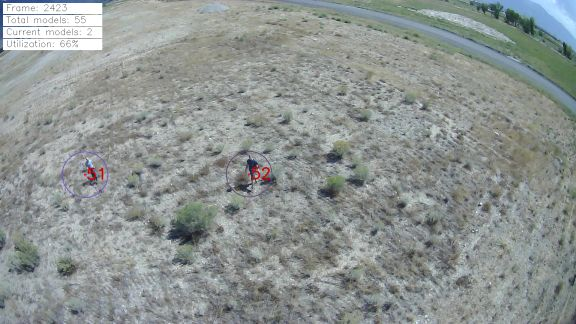
\includegraphics[width=0.95\textwidth]{images/chapter3/ID51_track_begin.png}
		\caption{Track ID 51 initiated by R-RANSAC tracker (t=0s)}
		\label{camera1}
	\end{subfigure}
	\begin{subfigure}{0.48\linewidth}
		\centering
		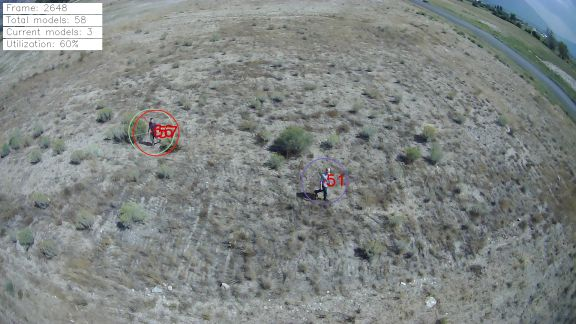
\includegraphics[width=0.95\textwidth]{images/chapter3/ID51_follow_begin.png}
		\caption{Human operator commanded to follow track ID 51 (t=13s)}
		\label{camera2}
	\end{subfigure}
	\begin{subfigure}{0.48\linewidth}
		\centering
		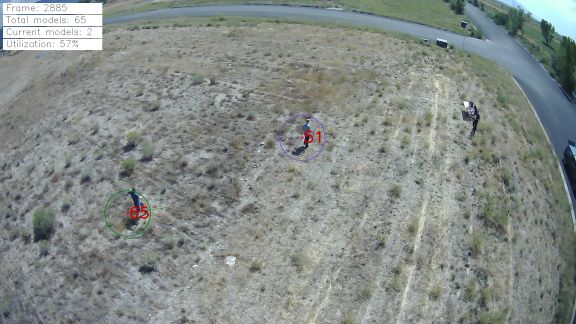
\includegraphics[width=0.95\textwidth]{images/chapter3/ID65_track_begin.png}
		\caption{Track ID 65 initiated by R-RANSAC tracker (t=27s)}
		\label{camera3}
	\end{subfigure}
	\begin{subfigure}{0.48\linewidth}
		\centering
		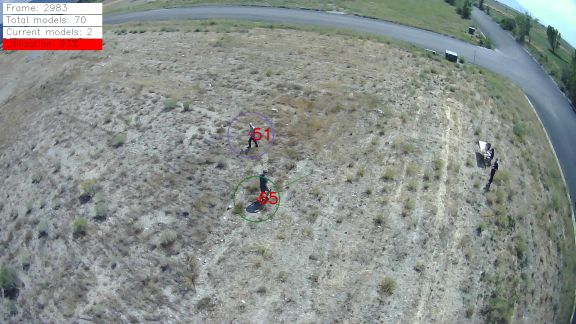
\includegraphics[width=0.95\textwidth]{images/chapter3/ID65_follow_begin.png}
		\caption{Human operator commanded to follow track ID 65 (t=35s)}
		\label{camera4}
	\end{subfigure}
	\centering
	\begin{subfigure}{0.48\linewidth}
		\centering
		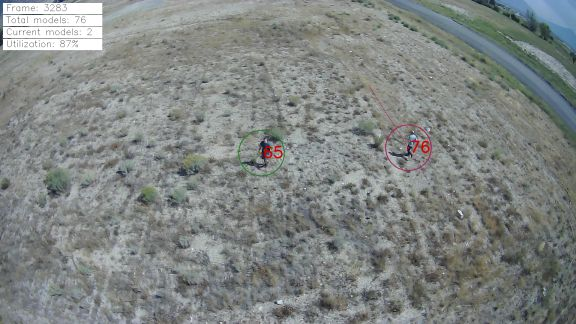
\includegraphics[width=\textwidth]{images/chapter3/ID65_following.png}
		\caption{A snapshot of the track ID 65 being followed (t=60s)}
		\label{camera5}
	\end{subfigure}
	\caption{Camera view at various events during t=0-60s.}
	\label{camera}
\end{figure}
As shown in Figure \ref{camera1}, the human operator sees this camera view of multiple moving objects being tracked from the ground station and commands the multirotor to follow a target of interest by sending the correct track ID (Figure \ref{camera2}). The hardware test lasted about 1 minute and in the middle (t=35s) the operator commanded the multirotor to follow a different target (Figure \ref{camera4}). Until another track ID given from the operator, the multirotor keeps following the current assigned target (Figure \ref{camera5}).

Figure \ref{image1} and \ref{image2} show the effort of the multirotor trying to place the target being followed in the center of image plane. In Figure \ref{image1} and Figure \ref{image2}, the numbered events listed in Figure \ref{camera} are illustrated in the image plane. A track with ID 51 is initialized by the R-RANSAC tracker, and later the multirotor was commanded to follow track 51. The R-RANSAC tracker detected another moving object in the camera field of view and started to track the object with ID 65 while the multirotor was still following the track 51. After a while, the human operator switches the target of interest resulting in the multirotor following track 65. The multirotor kept following the track 65 for the rest of experiment. Finally, Figure \ref{gps} illustrates the GPS coordinates of the multirotor to show its movement and heading during the experiment. 

\begin{figure}[htbp]
	\centering
	\framebox{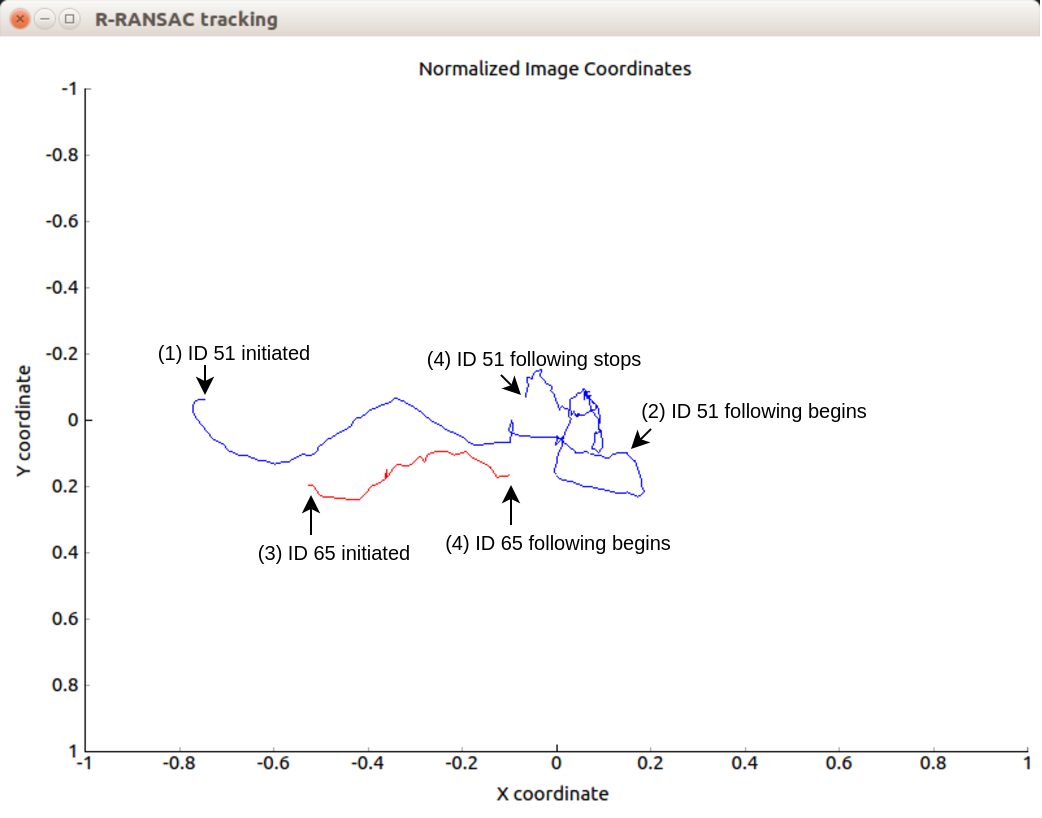
\includegraphics[height=7cm]{images/chapter3/ID65_follow_begin_annotated.png}}
	\caption{Tracks movement in the normalized image plane. Each event (1)-(4) corresponds to camera view in \ref{camera1}-\ref{camera4} respectively. Until the command to follow ID 65, the multirotor keeps the track ID 51 from leaving the camera view.}
	\label{image1}
\end{figure}

\begin{figure}[htbp]
	\centering
	\framebox{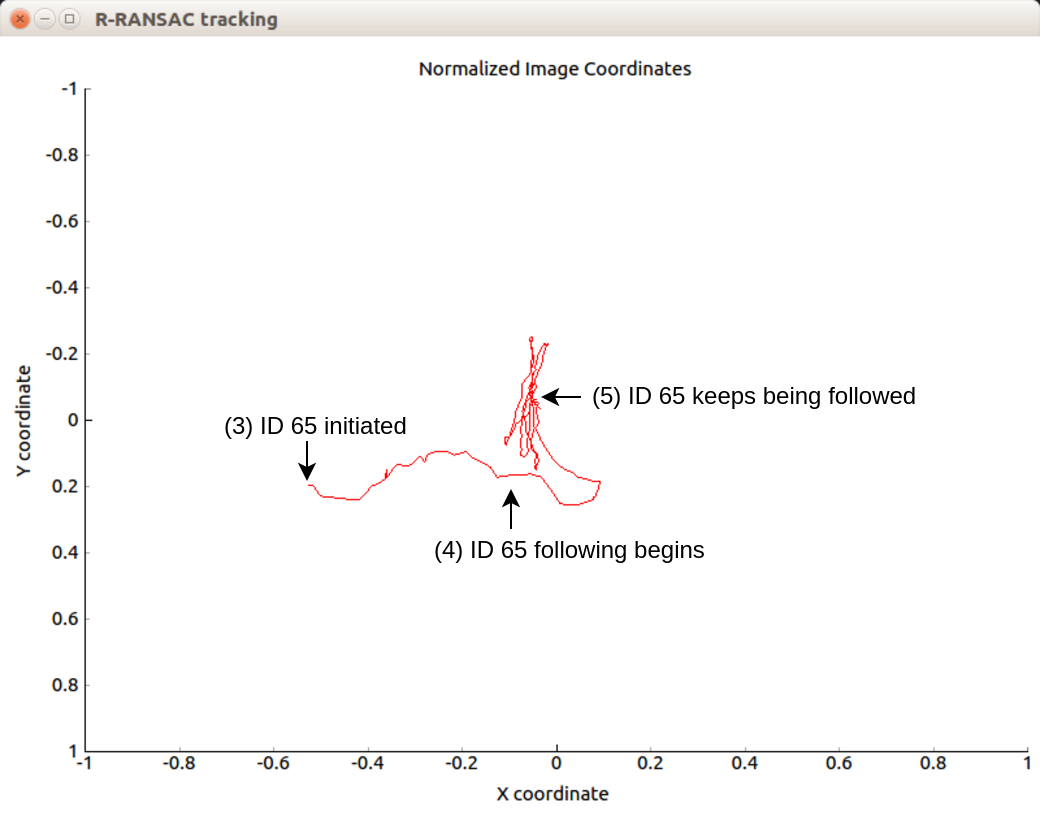
\includegraphics[height=7cm]{images/chapter3/ID65_trace_annotated.png}}
	\caption{The movement of track ID 65 in the normalized image plane. Each event (3)-(5) corresponds to camera view in \ref{camera3}-\ref{camera5} respectively. The controller keeps the track ID 65 in the camera field of view after receiving the command to do so from the human operator.}
	\label{image2}
\end{figure}

\begin{figure}[htbp]
	\centering
	\framebox{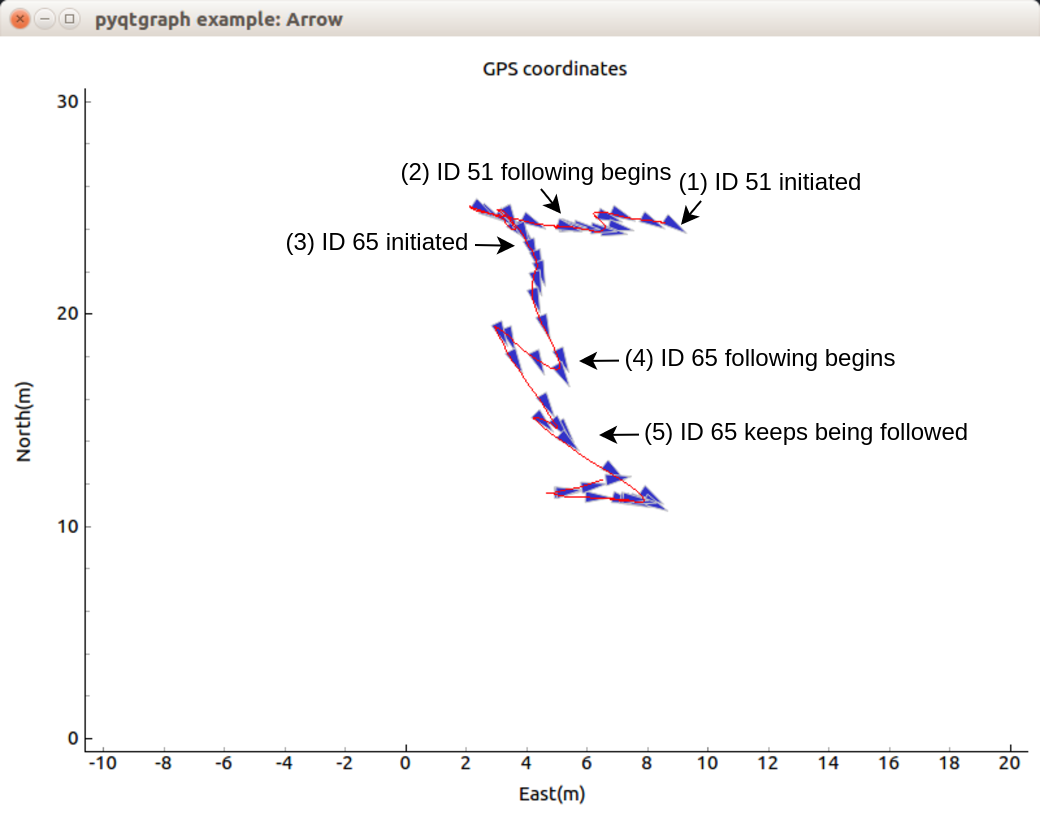
\includegraphics[height=7cm]{images/chapter3/GPS_trace.png}}
	\caption{Multirotor GPS footage and heading corresponding to camera view in \ref{camera1}-\ref{camera5} respectively.}
	\label{gps}
\end{figure}

\section{Conclusion}
In this work, a novel vision-based target following system with the R-RANSAC tracker is presented with hardware demonstration. The experimental result shows the feasibility of the real-time system in a realistic outdoor environment. With the R-RANSAC tracker, multiple moving objects in the camera view are tracked without having to know their colors or shapes. The controller is able to follow any particular target among the tracks with minimum effort to the human operator. The human operator is only expected to send a track ID number to the controller in order for the multirotor to follow the target of interest. This research opens up many other potential areas of research such as keeping multiple targets in the camera field of view, human machine interaction and multi UAS coordination in multiple target tracking situations.